\documentclass[border=8pt]{standalone}
\usepackage[T1]{fontenc}\usepackage[utf8]{inputenc}
\usepackage{helvet}\renewcommand{\familydefault}{\sfdefault}
\usepackage{tikz,xcolor}
\usetikzlibrary{arrows.meta,positioning,shapes.geometric,shapes.multipart,calc,fit,backgrounds,decorations.markings}
\definecolor{ink}{HTML}{1E1B16}\definecolor{paper}{HTML}{FBF8F2}\definecolor{clay}{HTML}{B5482A}\definecolor{soft}{HTML}{F1E9DA}\definecolor{pine}{HTML}{24402F}
\tikzset{
  every node/.style={font=\small,text=ink},
  >=Stealth, line/.style={draw=ink,line width=0.8pt},
  cls/.style={rectangle split,rectangle split parts=3,draw=ink,line width=0.8pt,fill=soft,align=left,inner xsep=6pt,inner ysep=4pt,
              rectangle split part align={center,left,left},minimum width=3.0cm},
  cls2/.style={rectangle split,rectangle split parts=2,draw=ink,line width=0.8pt,fill=soft,align=left,inner xsep=6pt,inner ysep=4pt,
              rectangle split part align={center,left},minimum width=3.0cm},
  box/.style={rectangle,draw=ink,line width=0.8pt,fill=soft,align=center,inner sep=5pt,minimum height=0.8cm},
  state/.style={rectangle,rounded corners=8pt,draw=ink,line width=0.8pt,fill=soft,align=center,inner sep=6pt,minimum width=2.2cm,minimum height=0.9cm},
  act/.style={rectangle,rounded corners=10pt,draw=ink,line width=0.8pt,fill=soft,align=center,inner sep=5pt,minimum width=2.4cm,minimum height=0.8cm},
  dec/.style={diamond,draw=ink,line width=0.8pt,fill=soft,inner sep=1pt,minimum width=0.9cm,minimum height=0.9cm},
  uc/.style={ellipse,draw=ink,line width=0.8pt,fill=soft,align=center,inner sep=3pt,minimum width=3.2cm,minimum height=1.0cm},
  note/.style={rectangle,draw=ink,line width=0.6pt,fill=yellow!12,align=left,inner sep=4pt,font=\footnotesize},
  lab/.style={font=\footnotesize,fill=paper,inner sep=1.5pt},
  err/.style={},
}
\newcommand{\actor}[3]{% x,y,label
  \draw[line width=0.8pt] (#1,#2+0.55) circle (0.17);
  \draw[line width=0.8pt] (#1,#2+0.38)--(#1,#2-0.15) (#1-0.3,#2+0.22)--(#1+0.3,#2+0.22) (#1,#2-0.15)--(#1-0.25,#2-0.6) (#1,#2-0.15)--(#1+0.25,#2-0.6);
  \node[font=\small] at (#1,#2-0.9) {#3};}
\begin{document}
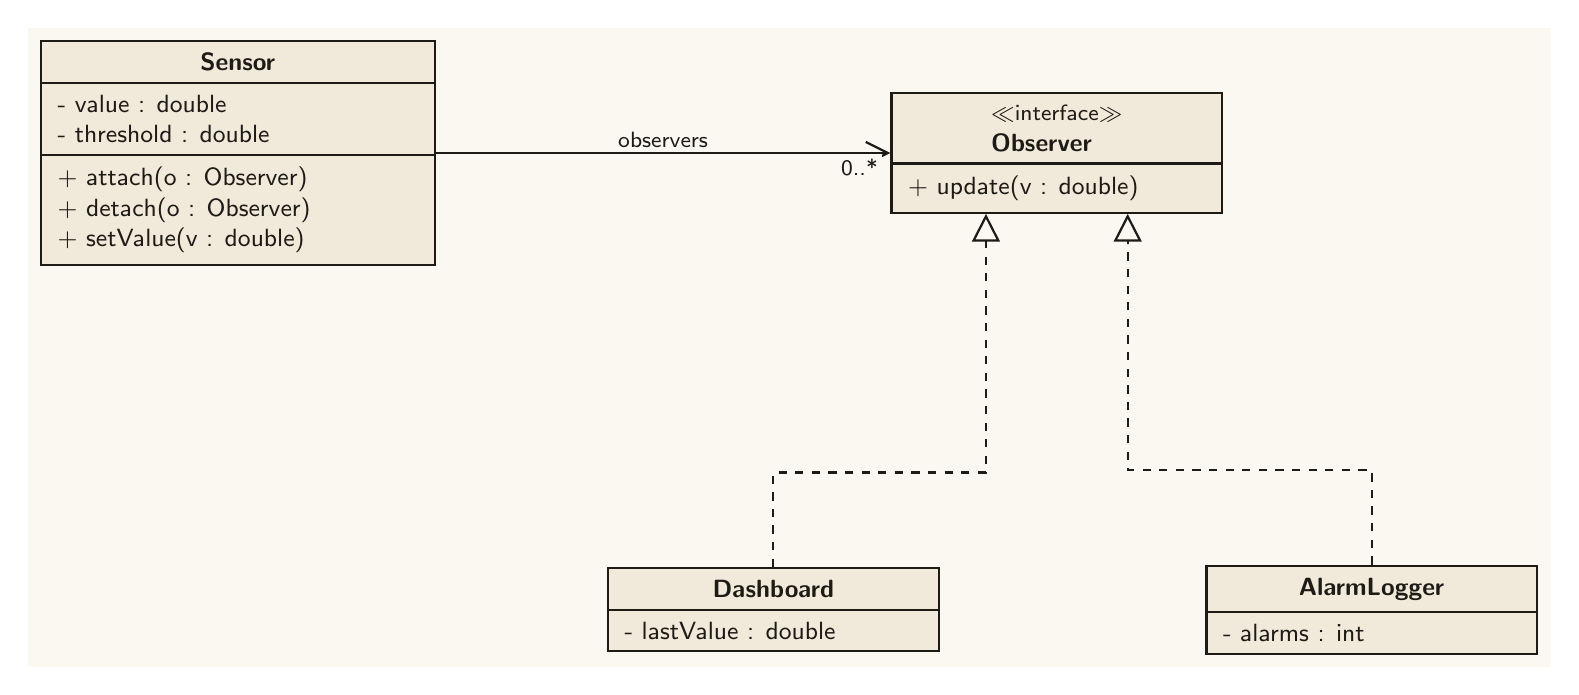
\begin{tikzpicture}[background rectangle/.style={fill=paper},show background rectangle]
\node[cls,minimum width=5.0cm] (Su) at (0,4.4) {\textbf{Sensor}\nodepart{two}- value : double\\- threshold : double\nodepart{three}+ attach(o : Observer)\\+ detach(o : Observer)\\+ setValue(v : double)};
\node[cls2,minimum width=4.2cm] (Ob) at (10.4,4.4) {{\footnotesize $\ll$interface$\gg$}\\ \textbf{Observer}\nodepart{two}+ update(v : double)};
\node[cls2,minimum width=4.2cm] (Da) at (6.8,-1.4) {\textbf{Dashboard}\nodepart{two}- lastValue : double};
\node[cls2,minimum width=4.2cm] (Al) at (14.4,-1.4) {\textbf{AlarmLogger}\nodepart{two}- alarms : int};
\draw[line,-{Straight Barb[length=8pt,width=8pt]}] (Su.east)--(Ob.west) node[midway,above,lab]{observers};
\node[lab,anchor=south east] at ([xshift=-0.1cm,yshift=-0.35cm]Ob.west) {0..*};
\draw[line,dashed,-{Triangle[open,length=10pt,width=10pt]}] (Da.north)--++(0,1.2)-|([xshift=-0.9cm]Ob.south);
\draw[line,dashed,-{Triangle[open,length=10pt,width=10pt]}] (Al.north)--++(0,1.2)-|([xshift=0.9cm]Ob.south);
\end{tikzpicture}
\end{document}
